\documentclass[tikz,border=10pt]{standalone}
\usepackage[scaled=0.95]{helvet}
\renewcommand{\familydefault}{\sfdefault}
\usepackage[europeanresistors,americanvoltages]{circuitikz}
\usetikzlibrary{arrows.meta,positioning}
\definecolor{TEJNavy}{HTML}{1E2B55}
\definecolor{TEJBlue}{HTML}{1769AA}
\definecolor{TEJGold}{HTML}{D49B19}
\definecolor{TEJRed}{HTML}{A43737}
\begin{document}
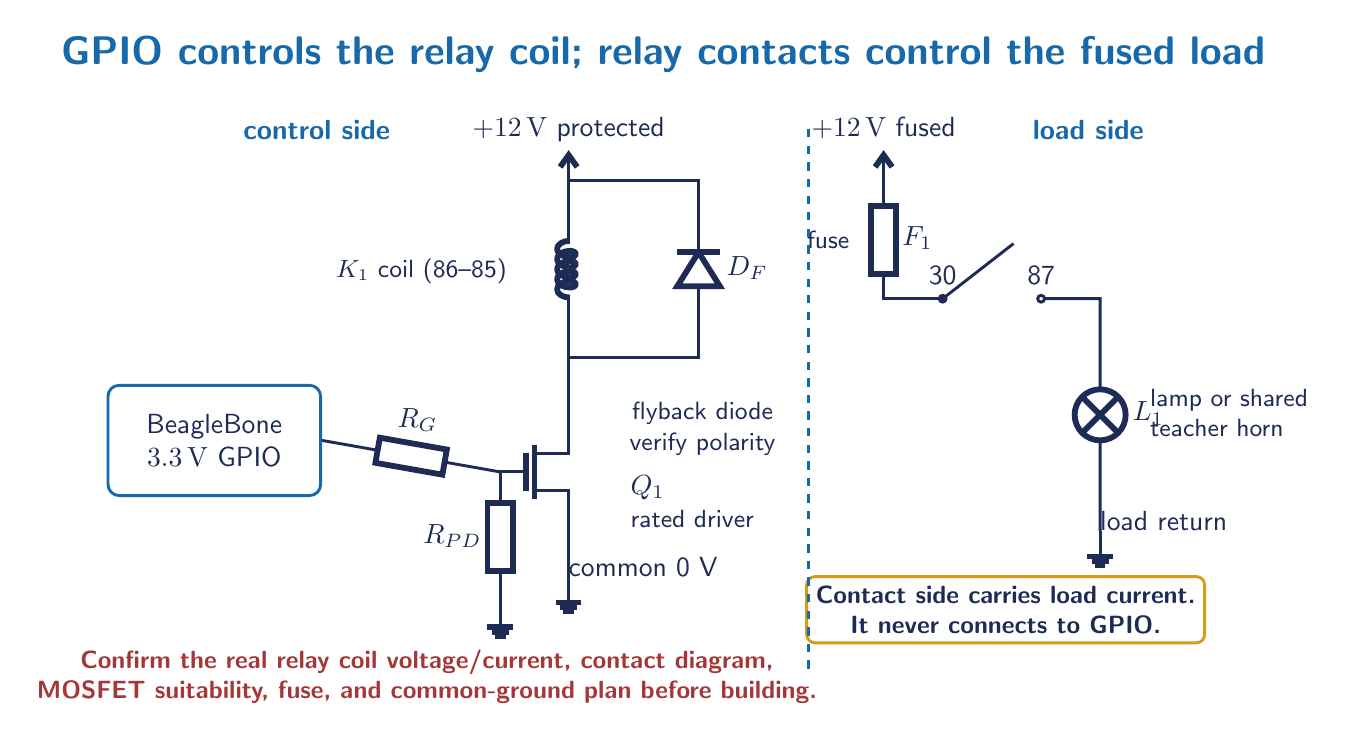
\begin{tikzpicture}[line width=1.05pt,draw=TEJNavy,text=TEJNavy,font=\sffamily]
  \ctikzset{bipoles/length=1.08cm}
  \node[font=\bfseries\Large,text=TEJBlue] at (7.2,8.05)
    {GPIO controls the relay coil; relay contacts control the fused load};

  % GPIO and MOSFET driver
  \node[draw=TEJBlue,rounded corners=4pt,minimum width=2.7cm,minimum height=1.4cm,align=center]
    (bbb) at (1.5,3.15) {BeagleBone\\$3.3\,\mathrm{V}$ GPIO};
  \node[nmos,scale=1.15] (Q1) at (6.0,2.75) {};
  \node[anchor=west] at (6.65,2.55) {$Q_1$};
  \node[anchor=west,font=\small] at (6.65,2.15) {rated driver};
  \draw (bbb.east) to[R,l={$R_G$}] (Q1.G);
  \draw (Q1.G) to[R,l_={$R_{PD}$}] ++(0,-1.65) node[ground] {};
  \draw (Q1.S) -- ++(0,-0.65) node[ground] {common 0 V};

  % Relay coil and flyback diode
  \coordinate (coilbottom) at (6.0,4.2);
  \coordinate (coiltop) at (6.0,6.45);
  \draw (Q1.D) -- (coilbottom)
    to[L] (coiltop)
    node[vcc] {$+12\,\mathrm{V}$ protected};
  \node[anchor=east,font=\small] at (5.35,5.3) {$K_1$ coil (86--85)};
  \draw (coilbottom) -- (7.65,4.2)
    to[D,l_={$D_F$}] (7.65,6.45) -- (coiltop);
  \node[font=\small,align=center] at (7.7,3.3) {flyback diode\\verify polarity};

  % Contact/load circuit kept separate
  \draw (10.0,6.45) node[vcc] {$+12\,\mathrm{V}$ fused}
    to[R,l={$F_1$}] (10.0,4.95)
    -- (10.75,4.95) node[circ,label=above:{30}] {};
  \node[anchor=east,font=\small] at (9.7,5.7) {fuse};
  \draw (10.75,4.95) -- (11.65,5.65);
  \draw (12.0,4.95) node[ocirc,label=above:{87}] {} -- (12.75,4.95)
    to[lamp,l={$L_1$}] (12.75,2.0)
    node[ground] {load return};
  \node[anchor=west,align=left,font=\small] at (13.25,3.5) {lamp or shared\\teacher horn};
  \node[draw=TEJGold,rounded corners=3pt,align=center,font=\bfseries\small]
    at (11.55,1.0) {Contact side carries load current.\\It never connects to GPIO.};

  \draw[dashed,TEJBlue,line width=1.1pt] (9.05,0.25) -- (9.05,7.1);
  \node[font=\bfseries,text=TEJBlue] at (2.8,7.1) {control side};
  \node[font=\bfseries,text=TEJBlue] at (12.6,7.1) {load side};
  \node[text=TEJRed,font=\bfseries\small,align=center] at (4.2,0.15)
    {Confirm the real relay coil voltage/current, contact diagram,\\MOSFET suitability, fuse, and common-ground plan before building.};
\end{tikzpicture}
\end{document}
